%% LyX 2.2.3 created this file.  For more info, see http://www.lyx.org/.
%% Do not edit unless you really know what you are doing.
\documentclass[english]{article}
\usepackage[T1]{fontenc}
\usepackage[utf8]{luainputenc}
\usepackage{geometry}
\geometry{verbose,tmargin=2cm,bmargin=2cm,lmargin=2cm,rmargin=2cm,headheight=2cm,headsep=2cm}
\setlength{\parindent}{0bp}
\usepackage{float}
\usepackage{amssymb}
\usepackage{graphicx}

\makeatletter

%%%%%%%%%%%%%%%%%%%%%%%%%%%%%% LyX specific LaTeX commands.
%% Because html converters don't know tabularnewline
\providecommand{\tabularnewline}{\\}

\makeatother

\usepackage{babel}
\begin{document}

\section{Comportamiento de Amplificador Operacional Inversor}

A lo largo de esta seccion se procedera a analizar el comportamiento
ideal y real del amplificador operacional \emph{LM324 }conectado como
se muestra en la figura \ref{1_a_1}. Considerando los valores de
los componentes como se puede ver en la tabla \ref{1_a_t_1}.

\begin{figure}[H]
\begin{centering}
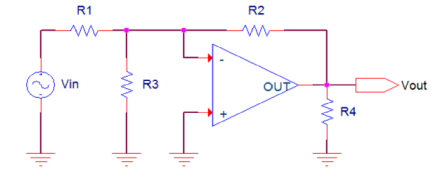
\includegraphics[scale=0.75]{Resources1a/Circuito1a}
\par\end{centering}
\caption{Circuito a analizar}
\label{1_a_1}
\end{figure}

\begin{table}[H]
\begin{centering}
\begin{tabular}{|c|c|c|c|}
\hline 
Caso & $R_{1}=R_{3}$ & $R_{2}$ & $R_{4}$\tabularnewline
\hline 
\hline 
1 & $10\left(k\Omega\right)$ & $100\left(k\Omega\right)$ & $40\left(k\Omega\right)$\tabularnewline
\hline 
2 & $10\left(k\Omega\right)$ & $10\left(k\Omega\right)$ & $40\left(k\Omega\right)$\tabularnewline
\hline 
3 & $100\left(k\Omega\right)$ & $10\left(k\Omega\right)$ & $400\left(k\Omega\right)$\tabularnewline
\hline 
\end{tabular}
\par\end{centering}
\caption{Valores de los componentes}
\label{1_a_t_1}

\end{table}

\subsection{Transferencia}

Comenzando por el analisis ideal, se pidió calcular y graficar la
relación $\frac{V_{out}}{V_{in}}$, esto quiere decir, considerando
$a_{0}$ finito y $A(\omega)$ con polo dominante. Considerando las
siguientes ecuaciones descriptas a continuacion y operando correctamente,
se llega a que la relacion $\frac{V_{out}}{V_{in}}$ esta dada por
la ecuación (\ref{eq:1_a_1}).

\[
\left\{ \begin{array}{c}
V_{out}=-A(\omega)v^{-}\\
I=i_{3}+i_{1}\\
i_{1}=-i_{2}\\
v^{-}=i_{3}R_{3}\\
V_{in}-IR_{1}=v^{-}
\end{array}\right.
\]

\begin{equation}
H(s)=\frac{V_{out}}{V_{int}}=\frac{\frac{a_{0}R_{3}R_{2}}{R_{1}R_{2}+2R_{3}R_{1}-R_{3}R_{2}}}{1+\frac{s}{\omega_{p}\left(\frac{R_{1}R_{2}+2R_{3}R_{1}-R_{3}R_{2}}{R_{1}R_{2}+R_{3}R_{1}-R_{3}R_{2}}\right)}}\label{eq:1_a_1}
\end{equation}

Como podemos ver, tenemos un polo en nuestra transferencia por lo
cual, el circuito se deberia comportar a grandes rasgos como un pasabajos.
Es importante notar, que el valor de $R_{4}$ no afecta a la transferencia
del circuito. Si graficamos la transferencia de el circuito para los
distintos casos, podemos ver que, en efecto, se comporta como un pasabajos,
con diferente frecuencia de corte $f_{0}$, esto se puede ver en la
figura \ref{1_a_2}.

\begin{figure}[H]
\begin{centering}
\includegraphics[scale=0.5]{\string"Resources1a/transferencias a(w)\string".pdf}
\par\end{centering}
\caption{Comportamiento del circuito para los diferentes valores de impedancias}
\label{1_a_2}CHEQUEARR SI STO ESTA BIENN
\end{figure}

\subsection{Impedancia de entrada}

Consecuentemente, se nos instó a calcular la impedancia de entrada
vista por el generador hacia nuestro circuito. Nuevamente, utilizando
las ecuaciones descriptas en la previa subseccion, y operando adecuadamente,
llegamos a que la impedancia de entrada es la descripta en la ecuación
(\ref{eq:1_a_2}).

\[
K=\frac{R_{2}a_{0}\omega_{p}(R_{3}+R_{1})-\omega_{p}(a_{0}-1)\left(R_{2}R_{3}+R_{1}R_{2}+R_{1}R_{3}\right)}{R_{2}a_{0}\omega_{p}-\left(R_{2}+R_{3}\right)\omega_{p}\left(a_{0}-1\right)}
\]

\[
C=\frac{\omega_{p}(a_{0}-1)\left(R_{2}R_{3}+R_{1}R_{2}+R_{1}R_{3}\right)-R_{2}a_{0}\omega_{p}\left(R_{3}+R_{1}\right)}{\left(R_{2}R_{3}+R_{1}R_{2}+R_{1}R_{3}\right)}
\]

\[
L=\frac{\left(R_{2}+R_{3}\right)\omega_{p}\left(a_{0}-1\right)-R_{2}a_{0}\omega_{p}}{R_{2}+R_{3}}
\]

\begin{equation}
\Rightarrow Z_{in}=K\,\frac{1+\frac{s}{C}}{1+\frac{s}{L}}\label{eq:1_a_2}
\end{equation}

Graficando la impedancia de entrada con respecto a la frecuencia de
entrada, se puede ver en la figura \ref{1_a_3}, como va variando
dependiendo de la frecuencia, es decir, no permanece constante. Nuevamente,
podemos observar como esta impedancia no es afectada por $R_{4}$.

\begin{figure}[H]
\caption{Impedancia de entrada}
\label{1_a_3}

\end{figure}

\subsection{Consideraciones para utilizar un modelo lineal del OpAmp}

Consecuentemente, decidimos aclarar cuales son las consideraciones
para caracterizar a nuestro circuito de manera lineal. Para esto poseemos
varias consideraciones que son descriptas a continuación.

\subsubsection{Saturación}

Si tenemos en cuenta un OpAmp ideal, nuestro primer contacto con un
circuito alineal se da cuando se entra en saturación, es decir, $\left|V_{out}\right|>\left|V_{cc}\right|$.
Si consideramos una tension de entrada de la forma $V_{in}=sin(2\pi ft)$,
es decir, con amplitud \emph{1(V)} \emph{, }solo nos basta con analizar
el valor del modulo de la transferencia vista en la ecuación (\ref{eq:1_a_1}).

\[
\left|H(f)\right|=\frac{\left|{R_{2}}\right|\left|{R_{3}}\right|\left|{a_{0}}\right|\left|\omega_{p}\right|\left|{R_{1}R_{2}+R_{1}R_{3}-R_{2}R_{3}}\right|}{\sqrt{4\pi^{2}f^{2}\left(R_{1}R_{2}+2R_{1}R_{3}-R_{2}R_{3}\right)^{2}+\omega_{p}^{2}\left(R_{1}R_{2}+R_{1}R_{3}-R_{2}R_{3}\right)^{2}}\left|{R_{1}R_{2}+2R_{1}R_{3}-R_{2}R_{3}}\right|}\leq V_{cc}
\]

\[
K=R_{1}R_{2}+2R_{1}R_{3}-R_{2}R_{3}
\]

\[
L=R_{1}R_{2}+R_{1}R_{3}-R_{2}R_{3}
\]

\[
f\geq\frac{\sqrt{-\left(V_{cc}\omega_{p}L\left|K\right|-\left|{R_{2}}\right|\left|{R_{3}}\right|\left|{a_{0}}\right|\left|{w}\right|\left|L\right|\right)\left(V_{cc}\omega_{p}\left(L\right)\left|K\right|+\left|{R_{2}}\right|\left|{R_{3}}\right|\left|{a_{0}}\right|\left|{w}\right|\left|L\right|\right)}}{2\pi\left(K\right)\left|{V_{cc}}\right|\left|K\right|}
\]

\[
\therefore\,f\geq26.5(kHz)\,Caso\,1
\]

\[
f\geq2.6(kHz)\,Caso\,2
\]

\[
f\geq265(Hz)\,Caso\,3
\]

\end{document}
